% arara: xelatex: {synctex: true}
% arara: indent: {overwrite: yes}
\documentclass[]{IMTexam}

\usepackage[enums]{IMTtikz}
\usepackage{cases}

\givecredits
\author{Isabella B.}
\USPN{11810773}
\date{}
\lecture{Física I} % disciplina
\lcode{CM0112}
\hwtype{Resolução} % o que é
\examname{Lista 1} % prova

\begin{document}

\maketitle

\begin{questions}

	\question Considere que os cossenos diretores $\alpha$, $\beta$ e $\gamma$ de um vetor são os tradicionais cossenos relacionados aos ângulos que este vetor possui em relação aos eixos coordenados $ x, y $ e $ z $. Prove que $\alpha^{2} + \beta^{2} + \gamma^{2} = 1$, usando geometria e álgebra vetorial.

	\begin{solution}
		Seja $ \vec{v} $ o vetor (não-nulo) que possui cossenos diretores $ \alpha, \beta $ e $\gamma$.

		\smallskip

		\begin{multi}
			Adotando as notações $ v=\enVert{v} $ e $ \vec{v}_i $ para a projeção ortogonal de um vetor $ \vec{v} $ sobre o eixo $ i $, e também assumindo a base canônica, temos
			\begin{gather*}
				v_x = v\,\alpha\\
				v_y = v\,\beta\\
				v_z = v\,\gamma
			\end{gather*}

			\nextcol

			e, portanto
			\begin{align*}
				v^{2}                                      & =v_x^{2}+v_y^{2}+v_z^{2}                                                   \\
				\implies\cancelto{1}{\dfrac{v^{2}}{v^{2}}} & =\dfrac{\del{v\,\alpha}^{2}+\del{v\,\beta}^{2}+\del{v\,\gamma}^{2}}{v^{2}} \\
				\implies\alpha^{2}+\beta^{2}+\gamma^{2}    & =1
			\end{align*}

		\end{multi}

		\hfill\qedsymbol
	\end{solution}

	\question Prove que as diagonais de um paralelogramo equilátero são perpendiculares.

	\begin{solution}

		\begin{multi}
			Seja $ ABCD $ um paralelogramo equilátero num plano cartesiano. Adotemos a base canônica $ \del{\ihat,\jhat} $.

			Posicionando o vértice $ A $ na origem $ O $ e a diagonal $ AC $ sobre o eixo $ x $, temos $ \ihat $ apontando na direção da diagonal.

			\nextcol

			\centering
			\begin{tikzpicture}[scale=2]
				\draw[->,black!60] (-0.5,0) -- (2,0) node[right] {$ x $};
				\draw[->,black!60] (0,-0.5) -- (0,0.75) node[above] {$ y $};

				\filldraw[blue!60,draw=black] (-30:0.25) -- (0,0) -- (30:0.25) arc (30:-30:0.25) node[midway,above right] {$ \alpha $} -- cycle;

				\draw (0,0) coordinate (O) -- ++(30:1) coordinate (B) -- ++(-30:1) coordinate (C) -- ++(30:-1) coordinate (D) -- cycle;

				\fill (O) circle (0.8pt) node[below left]  {$ A=O $};
				\fill (C) circle (0.8pt) node[below right] {$ C $};
				\fill (B) circle (0.8pt) node[above right] {$ B $};
				\fill (D) circle (0.8pt) node[below right] {$ D $};

				\draw[dashed] (O) -- (C) (B) -- (D);
				\draw[-Latex] (O) -- +(0.5,0) node[below] {$ \ihat $};
				\draw[-Latex] (O) -- node[left] {$ \jhat $} +(0,0.5);

			\end{tikzpicture}
		\end{multi}

		Seja $ \alpha $ o ângulo de abertura $ \angle BAD $ e $ l $ o comprimento de qualquer um de seus lados, temos $ B=(l\cos(\alpha/2),l\sin(\alpha/2)),D=(l\cos(\alpha/2),-l\sin(\alpha/2)) $ e o vetor $ \jhat $, portanto, aponta na direção da diagonal $ BD $ ($ \vec{BD}=D-B= (l\cos(\alpha/2)-l\cos(\alpha/2),-l\sin(\alpha/2)-l\sin(\alpha/2))=(0,-2l\sin(\alpha/2)) $, e não possui componente na horizontal).

		Como $ \ihat $ e $\jhat$ são perpendiculares (por definição), as diagonais de $ ABCD $ também o são.

		\hfill\qedsymbol

	\end{solution}

	\question Uma nave está subindo verticalmente sobre a superfície do planeta $ X $ cuja aceleração gravitacional é de \SI{2}{\meter\per\second\squared}. Quando se encontra a \SI{35}{\meter} de altura e tem uma velocidade de \SI{2}{\meter\per\second} repentinamente os motores se desligam. Qual é a rapidez em \si{\meter\per\second} com que ela se choca com o solo?

	\begin{solution}
		Adotemos um referencial com origem no solo e eixo vertical apontando para cima a partir de sua superfície. Seja a gravidade do planeta $ g=\SI{2}{\meter\per\second\squared} $, seja $ h=\SI{35}{\meter} $ a altura percorrida pela nave antes dela cair, seja $ a(t)=-g $ sua aceleração e $ v(0)=v_0=\SI{2}{\meter\per\second} $ sua velocidade inicial.

		Sendo a velocidade da nave no tempo a integral de sua aceleração
		\begin{align}
			v(t) & =\int a(t)\dif t=-g\,t+C_1,\quad C_1\in\mathbb{R}\nonumber \\
			\intertext{como $ v(t=0)=v_0 $, temos $ v_0=C $, e}
			v(t) & =-g\,t+v_0.\label{eq:vtss}
		\end{align}

		Integrando $ v(t) $ temos o deslocamento da nave
		\begin{align}
			y(t) & =\int v(t)\dif t=-\dfrac{1}{2}g\,t^{2}+v_0\,t+C_2,\quad C_2\in\mathbb{R}\nonumber \\
			\intertext{como $ y(t=0)=h $, temos $ C_2=h $, e}
			y(t) & =-\dfrac{1}{2}g\,t^{2}+v_0\,t+h.\label{eq:ytss}
		\end{align}

		Fazendo $ v(t)=v $ e isolando o tempo em \ref{eq:vtss}, temos
		\[ t=\dfrac{v_0-v}{g}, \]
		fazendo $ y(t)=y $ e substituindo em \ref{eq:ytss}, temos
		\begin{align}
			y           & =-\dfrac{1}{2}g\del{\dfrac{v_0-v}{g}}^{2}+v_0\del{\dfrac{v_0-v}{g}}+h\nonumber \\
			2g\del{y-h} & =\del{v_0-v}\del{v_0+v}\nonumber                                               \\
			%			2g\del{h-y}&=v^{2}-\cancel{2}v\,v_0+\cancel{v_0^{2}}+\cancel{v_0\,v}-\cancel{v_0^{2}}\nonumber\\
			v^{2}       & =v_0^{2}-2g\del{y-h},\label{eq:torrq3}
		\end{align}
		e, resolvendo para $ y=0 $, temos que a velocidade final na colisão da nave com o solo é \[  v=\sqrt{2^{2}-2\cdot2\cdot\del{0-35}}=\sqrt{4\del{1+35}}=\SI{12}{\meter\per\second}. \]
	\end{solution}

	\question Um elevador está subindo desde o chão com velocidade constante. No instante $ T_1 $ um homem deixa cair uma bola no chão. A bola cai com aceleração uniforme $ g $ e bate o solo no instante $ T_2 $. Encontre a altura do elevador no tempo $ T_1 $.

	\begin{solution}
		Fixando o sistema de coordenadas no chão, com o eixo vertical apontando para cima, sejam $ a(t)=-g $ a aceleração da bola no tempo, $ v(0)=v_0 $ sua velocidade inicial (idem à velocidade do elevador) e $ h_0 $ sua altura inicial (no momento $ T_1 $), podemos encontrar a função $ y(t) $ que descreve sua altura no tempo integrando a aceleração duas vezes:
		\begin{align*}
			y(t) & =\int v(t)\dif t=\int\int a(t) \dif t\dif t                                    \\
			     & =\int -g\,t+C_1\dif t,\quad C_1\in\mathbb{R}                                   \\
			\intertext{onde $ C_1=v_0 $ pelas condições iniciais da velocidade}
			y(t) & =\int -g\,t+v_0\dif t=-\dfrac{1}{2}g\,t^{2}+v_0\,t+C_2,\quad C_2\in\mathbb{R}.
		\end{align*}
		Pelas condições iniciais da posição, temos
		\begin{align*}
			y(T_1)=h & =-\dfrac{1}{2}g\,T_1^{2}+v_0\,T_1+C_2 \\
			C_2      & =\dfrac{1}{2}g\,T_1^{2}-v_0\,T_1+h,
		\end{align*}
		portanto,
		\begin{equation}\label{eq:ytbe}
			y(t)=-\dfrac{1}{2}g\del{t^{2}-T_1^{2}}+v_0\del{t-T_1}+h.
		\end{equation}

		Como $ y(t=T_2)=0 $, temos que a altura inicial do elevador será dada por
		\begin{align*}
			0 & =-\dfrac{1}{2}g\del{T_2^{2}-T_1^{2}}+v_0\del{T_2-T_1}+h \\
			h & =\del{T_2-T_1}\del{\dfrac{1}{2}g\del{T_2+T_1}-v_0}.
		\end{align*}
	\end{solution}

	\question Um jogador de basquete quer encestar a bola levantando-a desde uma altura de \SI{2}{\meter} do chão, com velocidade inicial de \SI{7}{\meter\per\second}. A distância da bola à vertical que passa pelo centro do cesto é de \SI{3}{\meter}, e o aro do cesto está a \SI{3.05}{\meter} de altura do chão. Em que ângulo a bola deve ser levantada?

	\begin{solution}
		Fixando a origem do sistema de coordenadas na posição inicial da bola (mãos do jogador), onde o eixo horizontal $ x $ aponta no sentido do cesto e é paralelo ao solo e o eixo vertical $ y $ aponta para cima (perpendicular ao solo), sejam a velocidade inicial da bola $ \vec{v_0} $, de módulo $ v_0=\SI{7}{\meter\per\second} $, $ \vec{g} $ a aceleração da gravidade, $ h=\num{3.05}-2=\SI{1.05}{\meter\per\second} $ a distância que deve ser percorrida pela bola na vertical, $ s=\SI{3}{\meter} $ a distância que deve ser percorrida pela bola na horizontal e $ \theta $ o ângulo formado pela velocidade inicial da bola com o solo.

		Podemos decompor a velocidade inicial da bola em suas componentes horizontal e vertical, adotando as notações $ v_{0x}=v_0\cos\theta $ para sua componente horizontal e $ v_{0y}=v_0\sin\theta $ para sua componente vertical.

		Para encontrar a função de sua posição na horizontal, basta integrar a respectiva componente da velocidade:
		\begin{align}
			x(t) & =\int v_{0x}\dif t=v_0\cos\theta\,t+C_1\quad C_1\in\mathbb{R} \\
			\intertext{pelas condições iniciais de posição, $ C_1=0 $, portanto}
			x(t) & =v_0\cos\theta\,t\label{eq:xtbb}
		\end{align}

		Podemos encontrar a função de sua velocidade na vertical integrando a aceleração:
		\begin{align}
			v_y(t) & =\int -g\dif t=\int -g\,t + C_2,\quad C_2\in \mathbb{R}\nonumber   \\
			\intertext{pelas condições iniciais da velocidade, $ C_2= v_{0y}$, portanto}
			v_y(t) & =\int -g\dif t=\int -g\,t + v_{0y}.\label{eq:vtbb}                 \\
			\intertext{e sua posição na vertical será dada por}
			y(t)   & =\int -g\,t+v_0\sin\theta \dif t                                   \\
			       & =-\dfrac{1}{2}g\,t^{2}+v_0\sin\theta\,t+C_3,\quad C_3\in\mathbb{R} \\
			\intertext{e, pelas condições iniciais temos $ C_3=0 $, portanto}
			y(t)   & =-\dfrac{1}{2}g\,t^{2}+v_0\sin\theta\,t\label{eq:ytbb}
		\end{align}

		Fazendo $ x(t)=s $ e isolando $ t $ em \ref{eq:xtbb}
		\[ x=v_0\cos\theta\,t\implies t=\dfrac{x}{v_0\cos\theta}, \]
		fazendo $ y(t)=h $ e substituindo em \ref{eq:ytbb}, temos
		\begin{align*}
			-\dfrac{1}{2}g\del{\dfrac{s}{v_0\cos\theta}}^{2}+v_0\sin\theta\del{\dfrac{s}{v_0\cos\theta}}    & =h  \\
			-\dfrac{1}{2}g\del{\dfrac{s}{v_0}}^{2}\dfrac{1}{\cos^{2}\theta}+s\dfrac{\sin\theta}{\cos\theta} & =h  \\
			\intertext{substituindo $ \sec^{2}\theta=1+\tan^{2}\theta $,\footnote{
					Pela relação fundamental da trigonometria segue que $ \sin^{2}\theta+\cos^{2}\theta=1\implies \tan^{2}\theta+1=1/\cos^{2}\theta=\sec^{2}\theta $.
				} temos}
			\tan^{2}\theta-2\dfrac{v_0^{2}}{g\,s}\tan\theta+2\dfrac{h}{g}\del{\dfrac{v_0}{s}}^{2}+1         & =0. \\
			\intertext{Fazendo $ \tan\theta=z $, recaímos sobre uma equação quadrátrica:}
			z^{2}-2\dfrac{v_0^{2}}{g\,s}z+\del{2\dfrac{h}{g}\del{\dfrac{v_0}{s}}^{2}+1}                     & =0. \\
		\end{align*}
		Tomando $ m=v_0^{2}/\del{g\,s} $ e como
		\[ \del{2\dfrac{h}{g}\del{\dfrac{v_0}{s}}^{2}+1}=(m+d)(m-d)\implies d=\sqrt{\del{\dfrac{v_0^{2}}{g\,s}}^{2}-\del{2\dfrac{h}{g}\del{\dfrac{v_0}{s}}^{2}+1}}, \]
		temos as raízes
		\begin{align*}
			m\pm d     & =\dfrac{v_0^{2}\pm\sqrt{\del{v_0^{2}}^{2}-\del{2h\,g\,v_0^{2}+\del{s\,g}^{2}}}}{s\,g},
			\intertext{substituindo os valores dados e tomando $ g=\SI{9.8}{\meter\per\second\squared} $, temos}
			z          & =\dfrac{7^{2}\pm\sqrt{7^{4}-\del{2\cdot\num{1.05}\cdot\num{9.8}\cdot7^{2}+(3\cdot\num{9.8})^{2}}}}{3\cdot\num{9.8}} \\
			\tan\theta & \approx\dfrac{49\pm\num{23}}{\num{29.4}}                                                                            \\
			\intertext{aplicando o $ \arctan $ de ambos os lados, temos, para $ 0\leqslant\theta<\SI{\pi/2}{\radian} $}
			\theta     & \approx\ang{67.8}\quad\textup{ou}\quad\theta\approx\ang{41.5}.
		\end{align*}
	\end{solution}

	\question Um ponto move-se no plano $ xy $ segundo as expressões $ x = a\,t $ e $ y = a\,t\del{1 - \alpha\,t} $, onde $ a $ e $\alpha$ são constantes positivas, e $ t $ é o tempo. Encontre:

	\begin{parts}
		\part A equação da trajetória $ y(x) $ do ponto e faça o gráfico.

		\begin{solution}

			\begin{multi}
				Fazendo $ t=x/a $ e substituindo na expressão de $ y $, conseguimos $ y(x) $:
				\[ y(x)=a\dfrac{x}{a}\del{1-\alpha\dfrac{x}{a}}=x\del{1-\dfrac{\alpha\,x}{a}} \]

				\nextcol
				\centering

				\begin{tikzpicture}
					\begin{axis}[
							align =center,
							title={$ y\times x $},
							every axis y label/.style={at={(current axis.north west)},above=0mm,xshift=0mm},
							every axis x label/.style={at={(current axis.right of origin)},anchor=west},
							axis lines=middle,
							ylabel={$ y $},
							xlabel={$ x $},
							ticks=none,
							xmin=-5.5,xmax=5.5,
							ymin=-200,ymax=20
						]
						\addplot[black,domain=-5:5] {-x*x*10+x};
						%	\coordinate (A) at (axis cs:0,10);
					\end{axis}
				\end{tikzpicture}
			\end{multi}
		\end{solution}

		\part A velocidade $ v $ e a aceleração $w$ do ponto como funções do tempo.

		\begin{solution}
			Como temos duas expressões para posição do ponto, devemos derivá-las separadamente para encontrar as funções velocidade e aceleração, portanto, temos, na horizontal
			\begin{gather}
				v_x(t)=\dod{x}{t}(t)=a,\\
				w_x(t)=\dod[2]{x}{t}=\dod{v_x}{t}=0,\\
				\intertext{e na vertical}
				v_y(t)=\dod{y}{t}(t)=a\del{1-2\alpha\,t},\\
				w_y(t)=\dod[2]{y}{t}=\dod{v_y}{t}=-2a\,\alpha.
			\end{gather}
		\end{solution}

		\part O instante $ t_0 $ no qual o vetor velocidade forma um ângulo de $\pi/4$ com o vetor aceleração.

		\begin{solution}
			Seja $ \del{\ihat,\jhat} $ a base canônica, os vetores velocidade $ \vec{v} $ e aceleração $ \vec{w} $ serão dados por
			\begin{gather}
				\vec{v}=v_x\,\ihat+v_y\,\jhat\\
				\vec{w}=w_x\,\ihat+w_y\,\jhat
			\end{gather}

			Para que esses vetores formem um ângulo de $ \SI{\pi/4}{\radian} $ entre eles, devemos ter
			\begin{align*}
				\<\vec{v},\vec{w}>                           & =v_x\,w_x+v_y\,w_y=|\vec{v}||\vec{w}|\cos\pi/4                                                 \\
				a\,0+a(1-2\alpha\,t_0)\del{-2a\,\alpha}      & =\dfrac{\sqrt{2}}{2}\sqrt{a^{2}+\del{a-2\alpha\,a\,t_0}^{2}}\sqrt{0^{2}+\del{-2a\,\alpha}^{2}} \\
				-2\sqrt{2}a^{2}\,\alpha(1-2\alpha\,t_0)      & =\envert{a}\sqrt{1+\del{1-2\alpha\,t_0}^{2}}\envert{2a\,\alpha}                                \\
				%				\intertext{assumindo $ a>0,\alpha>0 $, temos}
				2\del{1-4\alpha\,t_0+\del{2\alpha\,t_0}^{2}} & =2-4\alpha\,t_0+\del{2\alpha\,t_0}^{2}                                                         \\
				\del{\alpha\,t_0-1}4\alpha\,t_0              & =0                                                                                             \\
				\implies t_0                                 & =0\quad\text{ou}\quad t_0=\dfrac{1}{\alpha}
			\end{align*}
		\end{solution}
	\end{parts}

	\question Uma pedra é lançada a partir de um telhado com uma velocidade $ V $ que forma um ângulo $\alpha$ com a horizontal e descreve uma trajetória parabólica como mostrado na figura \ref{fig:fig1}. Qual é a distancia $ h $ na qual a velocidade da pedra é igual a $ 3V $?

	\begin{figure}[H]
		\centering
		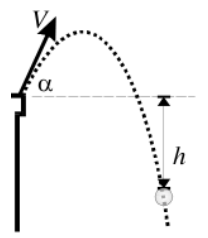
\includegraphics[height=0.25\textheight]{screenshot002}
		\caption{Lançamento oblíquo de uma pedra.}
		\label{fig:fig1}
	\end{figure}

	\begin{solution}
		Adotando o referencial com origem no telhado e dois eixos perpendiculares, vertical e horizontal, que apontam, respectivamente, para cima e para a direita, temos a decomposição da velocidade inicial em
		\begin{gather}
			V_{x}=V\cos\alpha,\label{eq:Vxr}\\
			V_{y}=V\sin\alpha.\label{eq:Vyr}
		\end{gather}

		Como o eixo vertical está sujeito à uma aceleração gravitacional $ -g $, temos a função de sua velocidade no tempo sendo dada por $ v_y(t)=\int -g\dif t=-g\,t+V_y $ (pela condição inicial). Dessa forma temos o vetor
		\[ \vec{v}(t)=V_x\,\ihat+v_y(t)\,\jhat \]
		e queremos encontrar o momento posterior onde possui velocidade $ 3V $, sendo, portanto, necessário analisar seu módulo:
		\begin{align*}
			\envert{\vec{v}(t)}=\sqrt{V_x^{2}+v_y^{2}}                                     & =3V           \\
			\intertext{substituindo \ref{eq:Vxr} e \ref{eq:Vyr} e fazendo $ t=t_h $, temos}
			\sqrt{\del{V\cos\alpha}^{2}+\del{V\sin\alpha-g\,t_h}^{2}}                      & =3V           \\
			V^{2}\del{\sin^{2}\alpha+\cos^{2}\alpha}-2V\,g\,t_h\sin\alpha+\del{g\,t_h}^{2} & =\del{3V}^{2} \\
			-2\del{2\dfrac{V}{g}}^{2}-2\dfrac{V}{g}\sin\alpha\,t_h+t_h^{2}                 & =0
		\end{align*}
		Resolvendo para $ t_h $, temos, por Bháskara,
		\begin{align*}
			t_h & =\dfrac{2(V/g)\sin\alpha\pm\sqrt{\del{2(V/g)\sin\alpha}^{2}+4\cdot2\del{2V/g}^{2}}}{2} \\
			t_h & =\dfrac{V}{g}\del{\sin\alpha\pm\sqrt{\sin^{2}\alpha+8}}
		\end{align*}
		Sendo a função analisada uma parábola, escolhemos o maior valor de $ t_h $, pois só nos interessa o momento onde $ |\vec{v}(t)|=3V $ e $ t>0 $.

		Para encontrar a altura $ h $ podemos integrar a velocidade vertical da pedra com respeito ao tempo e substituir $ t=t_h $, dessa forma temos
		\begin{align*}
			\int v_y(t)\dif t & =-\dfrac{1}{2}g\,t^{2}+V_y\,t=t\del{V_y-\dfrac{g\,t}{2}}                                                                               \\
			\intertext{substituindo $ t=t_h $, temos}
			h                 & =\del{\dfrac{V}{g}\del{\sin\alpha+\sqrt{\sin^{2}\alpha+8}}}\del{V\sin\alpha-\dfrac{g(V/g)\del{\sin\alpha+\sqrt{\sin^{2}\alpha+8}}}{2}} \\
			                  & =\dfrac{V^{2}}{2g}\del{\sin\alpha+\sqrt{\sin^{2}\alpha+8}}\del{\sin\alpha-\sqrt{\sin^{2}\alpha+8}}=\dfrac{\del{2V}^{2}}{g}
		\end{align*}
	\end{solution}

	\question Um canhão lança um projétil por cima de uma montanha de altura $ h $, de forma a passar quase tangenciando o cume $ C $ no ponto mais alto de sua trajetória.

	A distância horizontal entre o canhão e o cume é $ R $.

	\begin{figure}[H]
		\centering
		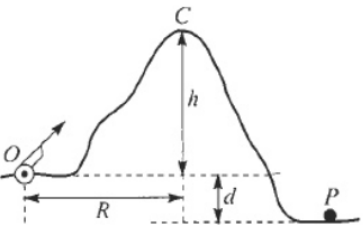
\includegraphics[width=0.5\linewidth]{screenshot003}
		\caption{Lançamento de projétil sobre uma montanha.}
		\label{fig:fig2}
	\end{figure}

	Atrás da montanha há uma depressão de profundidade d, figura \ref{fig:fig2}. Determine a distância horizontal entre o ponto de lançamento $ O $ e o ponto $ P $ onde o projétil atinge o solo, em função de $ R, d $ e $ h $.

	\begin{solution}
		Consideramos a origem o ponto $ O $ de lançamento do projétil, onde posicionaremos um eixo de coordenadas com os eixos $ y $ orientado para cima e $ x $ para a direita.

		Sendo o movimento parabólico uma função quadrática da forma \[ y(x)=a\,x^{2}+b\,x+c \]
		onde $ y $ é o deslocamento vertical e $ x $ é o deslocamento horizontal, derivando ambos os lados, temos
		\begin{align*}
			(y(x))' & =(a\,x^{2}+b\,x+c)' \\
			v_y(x)  & =2a\,x+b
		\end{align*}
		onde $ v_y $ é a projeção da velocidade no eixo $ y $.

		Seja $ v_{0y} $ a velocidade inicial projetada no eixo $ y $, montando dois sistemas com os valores conhecidos para $ v(x) $ e $ y(x) $, respectivamente, temos
		\begin{align*}
			 & \begin{cases}
				v_y(0)=b=v_{0y} \\
				v_y(R)=0\implies 2a\,R+v_{0y}=0\implies a=-\dfrac{v_{0y}}{2R}
			\end{cases} \\
			 & \begin{cases}
				y(0)=0\implies c=0 \\
				y(R)=h\implies -\dfrac{v_{0y}}{2R}\,R^{2}+v_{0y}\,R=h
			\end{cases}
		\end{align*}
		Resolvendo a última equação para $ v_{0y} $, temos
		\begin{align*}
			-\dfrac{v_{0y}}{2}\,R+v_{0y}\,R & =h \\
			\dfrac{v_{0y}}{2}\,R=h               \\
			v_{0y}=\dfrac{2h}{R}
		\end{align*}

		Portanto, $ y(x)=-\dfrac{v_{0y}}{2R}x^{2}+v_{0y}\,x\implies y(x)=-\dfrac{h}{R^{2}}x^{2}+2\dfrac{h}{R}x $.

		Resolvendo para $ y(x)=-d $, temos
		\begin{align*}
			-\dfrac{h}{R^{2}}x^{2}+2\dfrac{h}{R}x   & =-d \\
			-\dfrac{h}{R^{2}}x^{2}+2\dfrac{h}{R}x+d & =0
		\end{align*}

		\begin{multi}[2][t]

			por Bháskara
			\begin{align*}
				\Delta & =\del{2\dfrac{h}{R}}^{2}-4\del{-\dfrac{h}{R^{2}}}d \\
				       & =\dfrac{4}{R^{2}}h^{2}+\dfrac{4}{R^{2}}h\cdot d    \\
				       & =\dfrac{4}{R^{2}}\del{h^{2}+h\cdot d}
			\end{align*}
			\begin{align*}
				x & =\dfrac{-\dfrac{2h}{R}\pm\sqrt{\dfrac{4}{R^{2}}\del{h^{2}+h\cdot d}}}{2\del{-\dfrac{h}{R^{2}}}}
			\end{align*}

			\nextcol
			como $ x>0 $
			\begin{align*}
				x & =\dfrac{\cancel{\dfrac{2}{R}}h+\cancel{\dfrac{2}{R}}\sqrt{h^{2}+h\cdot d}}{\cancel{\dfrac{2}{R}}\cdot\dfrac{h}{R}} \\
				  & =\dfrac{R}{h}\del{h+\sqrt{h^{2}\del{1+d/h}}}                                                                       \\
				  & =R\del{1+\sqrt{1+\dfrac{d}{h}}}
			\end{align*}
		\end{multi}
	\end{solution}

	\question Uma roda pneumática segue em linha reta sem deslizar. Seu centro se move com velocidade constante $ v $. Uma pequena pedra alojada no extremo da roda toca o caminho em $ t = 0 $. Encontrar a posição, velocidade e aceleração da pedra como função do tempo.

	\begin{figure}[H]
		\centering
		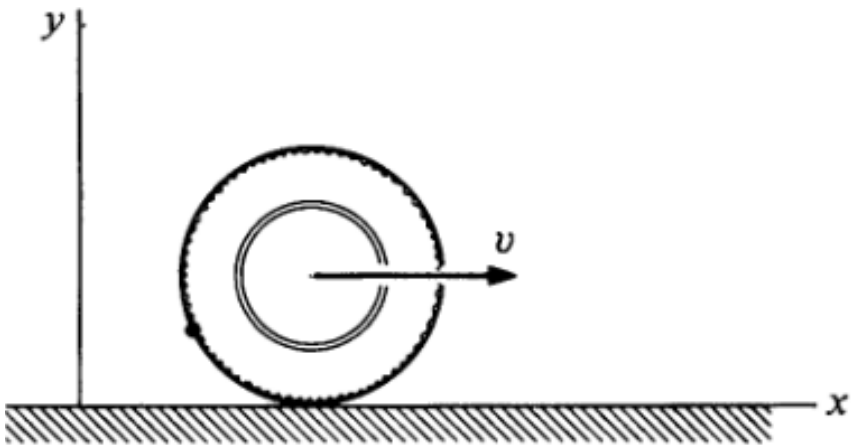
\includegraphics[width=0.5\linewidth]{screenshot004}
		\caption{Roda pneumática.}
		\label{fig:fig3}
	\end{figure}

	\begin{solution}
		Adotando o referencial do centro da roda, sabemos que a pedra não sofre ação da gravidade, mas possui uma aceleração radial $ \alpha $ que a mantém fixada em sua trajetória circular.

		Assumindo que a roda pneumática não desliza, seja seu raio $ r $, sua velocidade angular $ \omega $ e sua massa desprezível, pela condição de rolamento $ v=\omega\,r $, ou seja, sua extremidade deve se mover com velocidade igual àquela do seu centro. Sabemos também que a pedra se move de acordo com
		\begin{equation}\label{eq:rsiwr}
			\vec{r}(t)=A\sin(\omega\,t+\beta)\ihat+B\cos(\omega\,t+\beta)\jhat\quad\textup{(forma geral de um oscilador harmônico)}
		\end{equation}
		pelas condições iniciais, temos
		\[ \vec{r}(0)=0\,\ihat-r\,\jhat=A\sin(\beta)\ihat+B\cos(\beta)\jhat \]
		analisando as componentes, temos, para $ A\neq0 $,
		\begin{gather*}
			\begin{cases}
				A\sin\beta=0 \\
				B\cos\beta=-r
			\end{cases}\\
			\implies \beta=0\quad\textup{ou}\quad\beta=\pi
		\end{gather*}
		tomando $ \beta=0 $, temos $ B=-r $.

		Derivando $ \vec{r}(t) $, encontramos a função de sua velocidade no tempo
		\[ \vec{v}(t)=\dod{\vec{r}(t)}{t}=\dfrac{A\,v}{r}\cos\del{\dfrac{v\,t}{r}}\ihat+v\sin\del{\dfrac{v\,t}{r}}\jhat \]
		pela condição inicial da velocidade, temos
		\[ \vec{v}(0)=-v\,\ihat+0\,\jhat=\dfrac{A\,v}{r}\cos0\,\ihat+v\sin0\,\jhat\implies A=-r \]

		Derivando novamente, temos a função da aceleração da pedra no tempo
		\[ \vec{a}(t)=\dod{\vec{v}(t)}{t}=\dod[2]{\vec{r}(t)}{t}=\alpha\sin\del{\dfrac{v\,t}{r}}\ihat+\alpha\cos\del{\dfrac{v\,t}{r}}\jhat,\quad\textup{onde }\alpha=\dfrac{v^{2}}{r} \]

		\begin{multi}
			Realizando uma transformação de Galileu, adotamos o referencial externo, com origem na posição da pedra em $ t=0 $.

			\[ \vec{r}=\vec{r'}-\del{v\,t\,\ihat+r\,\jhat}\implies \vec{r'}=\vec{r}+\del{v\,t\,\ihat+r\,\jhat} \]
			%			da mesma forma, para a velocidade temos
			%			\[ \vec{v'}=\vec{v}+v\,\ihat \]
			\nextcol
			\centering
			\begin{tikzpicture}
				\coordinate (Si) at (0,0);
				\draw[->] (Si)++(-0.5,0) -- +(2,0);
				\draw[->] (Si)++(0,-0.5) -- +(0,2);
				\node[below left] at (Si) {Centro da roda};

				\coordinate (Sd) at (3,2);
				\draw[->] (Sd)++(-0.5,0) -- +(2,0);
				\draw[->] (Sd)++(0,-0.5) -- +(0,2);
				\node[below right] at (Sd) {Exterior};

				\coordinate (obj) at (1,3);
				\draw[-Latex] (Si) -- node[above left] {$ \vec{r} $} (obj);
				\draw[-Latex] (Sd) -- node[above right] {$ \vec{r'} $}(obj);
				\draw[-Latex] (Si) -- node[below right] {$ -\del{v\,t\,\ihat+r\,\jhat} $} (Sd);

				\filldraw (obj) circle (2pt) node[above] {Pedra};
			\end{tikzpicture}
		\end{multi}

		Portanto, temos
		\begin{align*}
			\vec{r'}(t) & =\del{v\,t-r\sin\del{\dfrac{v\,t}{r}}}\ihat+r\del{1-\cos\del{\dfrac{v\,t}{r}}}\jhat, \\
			\vec{v'}(t) & =v\del{1-\cos\del{\dfrac{v\,t}{r}}}\ihat+v\sin\del{\dfrac{v\,t}{r}}\jhat,            \\
			\vec{a'}(t) & =\alpha\sin\del{\dfrac{v\,t}{r}}\ihat+\alpha\cos\del{\dfrac{v\,t}{r}}\jhat.
		\end{align*}
	\end{solution}

	\question Um garoto se encontra no pico de uma montanha a qual tem um ângulo $\phi$ uniforme com a horizontal, como na figura \ref{fig:fig4}. A que ângulo $\theta$ da horizontal deveria ele lançar uma pedra tal que a distância percorrida seja a maior possível?

	\begin{figure}[H]
		\centering
		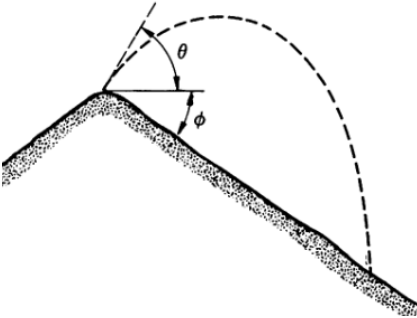
\includegraphics[width=0.4\linewidth]{screenshot001}
		\caption{Trajetória do lançamento oblíquo de uma pedra.}
		\label{fig:fig4}
	\end{figure}

	\begin{solution}
		Adotando o sistema de coordenadas com origem no ponto de lançamento da pedra e eixos horizontal e vertical orientados para a direita e para cima, respectivamente. Seja $ \vec{v}(t) $ a função da velocidade na pedra no tempo, $ \vec{r}(t) $ a função de sua posição, $ \vec{v_0} $ sua velocidade inicial e $ g $ o módulo da aceleração da gravidade.

		Temos que $ \vec{v}(t) $ será dado por
		\begin{equation}\label{eq:vt}
			\vec{v}(t)=\vec{v_0}+\int -g\,\jhat\dif t=\vec{v_0}-g\,t\,\jhat.
		\end{equation}

		De forma análoga, temos
		\begin{equation}\label{eq:rt}
			\vec{r}(t)=\int\vec{v_0}-g\,t\jhat\dif t=\vec{v_0}\,t-\dfrac{1}{2}g\,t^{2}\,\jhat.
		\end{equation}

		Pelo enunciado, queremos maximizar a componente horizontal da posição $ r_x $ na intercessão de $ \vec{r}(t) $ e da reta $ \vec{s}(t) $ (que descreve a descida da montanha). Para tanto, basta utilizarmos que a componente horizontal se conserva, e a vertical terá que descer uma altura adicional $ h=r_x\tan\phi $ além de retornar à altura inicial. Dessa forma, encontramos um tempo $ t=t_i $ (tempo de intercessão) fazendo
		\begin{align*}
			r_y=v_{0y}\,t_i-\dfrac{1}{2}g\,t_i^{2}        & =-h \\
			t_i^{2}-\dfrac{2}{g}v_{0y}\,t_i-\dfrac{2}{g}h & =0
		\end{align*}
		de tal forma que (por Bháskara), temos
		\[ t_i=\dfrac{(2v_{0y}/g)\pm\sqrt{(2v_{0y}/g)^{2}+4(2/g)h}}{2}=\dfrac{v_{0y}\pm\sqrt{v_{0y}^{2}+2g\,h}}{g} \]
		e, substituindo o maior valor (tempo posterior) em $ r_x $ temos
		\begin{align*}
			r_x(t_i)                                                                                & =r_{i}=v_{0x}\,t_i=v_0\,\cos\theta\del{\dfrac{v_{0y}+\sqrt{v_{0y}^{2}+2g(r_i\tan\phi)}}{g}} \\
			\del{r_i\dfrac{g}{v_0\cos\theta}-v_{0y}}^{2}                                            & =v_{0y}^{2}+2g(r_i\tan\phi)                                                                 \\
			r_i^{2}\del{\dfrac{g}{v_0\cos\theta}}^{2}-2g\,r_i\dfrac{v_{0}\sin\theta}{v_0\cos\theta} & =2g\,r_i\tan\phi                                                                            \\
			r_i^{2}-2\dfrac{\del{v_0\cos\theta}^{2}}{g}\del{\tan\phi+\tan\theta}r_i                 & =0                                                                                          \\
			r_i\del{r_i-2\dfrac{\del{v_0\cos\theta}^{2}}{g}\del{\tan\phi+\tan\theta}}               & =0
		\end{align*}
		\begin{multi}[2][t]
			para $ r_i\neq0 $, temos
			\begin{align*}
				r_i & =2\dfrac{\del{v_0\cos\theta}^{2}}{g}\del{\tan\phi+\tan\theta}                                               \\
				    & =2\dfrac{\del{v_0\cos\theta}^{2}}{g}\del{\dfrac{\sin\phi}{\cos\phi}+\dfrac{\sin\theta}{\cos\theta}}         \\
				    & =2\dfrac{\del{v_0\cos\theta}^{2}}{g}\del{\dfrac{\sin\phi\cos\theta+\sin\theta\cos\phi}{\cos\phi\cos\theta}} \\
				    & =\dfrac{v_0^{2}}{g\cos\phi}2\cos\theta\sin\del{\phi+\theta}                                                 \\
				\intertext{por \ref{eq:stp}}
				r_i & =\dfrac{v_0^{2}}{g\cos\phi}\del{\sin\del{2\theta+\phi}+\sin\phi}
			\end{align*}

			\nextcol

			Nota:
			\begin{align}
				\sin\del{a+b} &                &  & =\sin a\cos b+\sin b\cos a\nonumber \\
				              & +\sin\del{a-b} &  & =\sin a\cos b-\sin b\cos a\nonumber \\
				\sin\del{a+b} & +\sin\del{a-b} &  & =2\sin a\cos b\label{eq:stp}
			\end{align}
		\end{multi}

		\smallskip
		que deve ser maximizada (com respeito à $ \theta $) quando $ \dif r_i/\dif\theta=0 $, dessa forma
		\begin{align*}
			\dod{r_i}{\theta}=\dfrac{v_0^{2}}{g\cos\phi}\del{2\cos\del{2\theta+\phi}} & =0                                                       \\
			\cos\del{2\theta+\phi}                                                    & =0                                                       \\
			2\theta+\phi                                                              & =\dfrac{\pi}{2}\quad\implies\theta=\dfrac{\pi/2-\phi}{2}
		\end{align*}

		%	\begin{align*}
		%		\sin\theta\del{\sqrt{1-\del{v_0\cos\theta}^{2}}+v_0\sin\theta}&=v_0\cos^{2}\theta\del{v_0\sin\theta\del{1-\del{v_0\cos\theta}^{2}}^{-1/2}+1}\\
		%		v_0\del{\sin^{2}\theta-\cos^{2}\theta}&=\sin\theta\del{v_0^{2}\cos^{2}\theta\del{1-\del{v_0\cos\theta}^{2}}^{-1/2}-\del{1-\del{v_0\cos\theta}^{2}}^{1/2}}\\
		%%		\del{1-\del{v_0\cos\theta}^{2}}^{1/2}v_0\del{\sin^{2}\theta-\cos^{2}\theta}&=\sin\theta\del{v_0^{2}\cos^{2}\theta-\del{1-\del{v_0\cos\theta}^{2}}}\\
		%		\del{1-\del{v_0\cos\theta}^{2}}^{1/2}v_0\del{1-2\cos^{2}\theta}&=\sqrt{1-\cos^{2}\theta}\del{2\del{v_0\cos\theta}^{2}-1}\\
		%		\intertext{fazendo $ \cos^{2}\theta=z $ e elevando ao quadrado, temos}
		%		v_0^{2}\del{1-v_0^{2}\,z}\del{1-4z+4z^{2}}&=\del{1-z}\del{1-4v_0^{2}\,z+4v_0^{4}z^{2}}\\
		%%		\del{v_0^{2}-v_0^{4}\,z}\del{1-4z+4z^{2}}&=\del{1-z}\del{1-4v_0^{2}\,z+4v_0^{4}z^{2}}\\
		%%		
		%		v_0^{2}
		%		{\color{cyan}-\cancel{4v_0^{2}\,z}}+
		%		{\color{red}\cancel{4v_0^{2}\,z^{2}}}
		%		-v_0^{4}\,z
		%		+{\color{blue}\cancel{4v_0^{4}\,z^{2}}}
		%		{\color{green}-\cancel{4v_0^{4}\,z^{3}}}
		%		&=
		%		1
		%		{\color{cyan}-\cancel{4v_0^{2}\,z}}
		%		+{\color{red}\cancel{4v_0^{2}\,z^{2}}}
		%		-z
		%		+{\color{blue}\cancel{4v_0^{4}\,z^{2}}}
		%		{\color{green}-\cancel{4v_0^{4}\,z^{3}}}\\
		%%		
		%		\del{1-v_0^{4}}z&=\del{1-v_0^{2}}\\
		%		z&=\cos^{2}\theta=\dfrac{1}{\del{1+v_0^{2}}}\\
		%		\implies\cos\theta&=\envert{\dfrac{\sqrt{1+v_0^{2}}}{1+v_0^{2}}}\\
		%		\implies\theta&=\pm\arccos\del{\envert{\dfrac{\sqrt{1+v_0^{2}}}{1+v_0^{2}}}}.
		%	\end{align*}
		%
		%	Como $ \theta\geqslant0 $ e que maximiza a função, temos
		%	\[ \theta=\arccos\del{\dfrac{\sqrt{1+v_0^{2}}}{1+v_0^{2}}}. \]
	\end{solution}

\end{questions}
\end{document}
